\documentclass[12pt,a4paper]{ctexart}
\usepackage{amsmath,amssymb,bm}
\usepackage{graphicx}
\usepackage[margin=2.5cm]{geometry}
\usepackage{booktabs}
\usepackage{caption}
\graphicspath{{figures/}}

\title{\textbf{计算机控制系统设计与实践\\ 第四周作业}}
\author{}
\date{}

\begin{document}
\maketitle

\noindent
\begin{tabular}{@{}ll@{\hspace{3em}}ll@{}}
姓\quad 名：\underline{\hspace{6em}} & & 学\quad 号：\underline{\hspace{6em}} \\[1ex]
专\quad 业：\underline{\hspace{6em}} & & 指导教师：\underline{\hspace{6em}} \\
\end{tabular}

\bigskip
\hrule
\bigskip

\section{用后向差分法推导控制算法的离散化表达式}

\subsection{题目}
已知连续控制算法的传递函数
\begin{equation}
G(s)=\frac{Y(s)}{X(s)}=\frac{2\left(1+\dfrac{1}{5s}+2s\right)}{1+0.2s},
\qquad \text{控制周期 } T_s=1\,\mathrm{s},
\end{equation}
要求用\textbf{后向差分}（向后差分）法推导其离散化表达式（差分方程）。

\subsection{连续传递函数的整理}
先观察分子：$2\left(1+\dfrac{1}{5s}+2s\right)$ 具有 PID 控制器
$K_p\left(1+\dfrac{1}{T_i s}+T_d s\right)$ 的标准形式，其中比例系数 $K_p=2$、积分时间
$T_i=5$、微分时间 $T_d=2$；而 $\dfrac{1}{1+0.2s}$ 为一阶惯性（低通滤波）环节。将分子展开：
\begin{equation}
G(s)=\frac{2+\dfrac{0.4}{s}+4s}{1+0.2s}.
\end{equation}
分子、分母同乘以 $s$，化为关于 $s$ 的有理真分式：
\begin{equation}
G(s)=\frac{Y(s)}{X(s)}=\frac{4s^{2}+2s+0.4}{0.2s^{2}+s}.
\end{equation}

\subsection{后向差分变换}
后向差分法用一阶向后差商近似微分，即
\begin{equation}
\frac{\mathrm{d}e(t)}{\mathrm{d}t}\bigg|_{t=kT_s}\approx\frac{e(k)-e(k-1)}{T_s},
\end{equation}
对应到复域即用
\begin{equation}
s\;\longrightarrow\;\frac{1-z^{-1}}{T_s}
\end{equation}
替换传递函数中的 $s$。代入 $T_s=1$，得
\begin{equation}
s=1-z^{-1}.
\end{equation}

\subsection{代入并整理为 $z$ 传递函数}
将上述有理真分式交叉相乘：
\begin{equation}
Y(s)\left(0.2s^{2}+s\right)=X(s)\left(4s^{2}+2s+0.4\right).
\end{equation}
把 $s=1-z^{-1}$ 及 $s^{2}=(1-z^{-1})^{2}=1-2z^{-1}+z^{-2}$ 代入，分别整理左右两端的系数：
\begin{equation}
0.2s^{2}+s = 0.2\left(1-2z^{-1}+z^{-2}\right)+\left(1-z^{-1}\right)
            = 1.2-1.4z^{-1}+0.2z^{-2},
\end{equation}
\begin{equation}
4s^{2}+2s+0.4 = 4\left(1-2z^{-1}+z^{-2}\right)+2\left(1-z^{-1}\right)+0.4
            = 6.4-10z^{-1}+4z^{-2}.
\end{equation}
于是得到脉冲传递函数
\begin{equation}
G(z)=\frac{Y(z)}{X(z)}=\frac{6.4-10z^{-1}+4z^{-2}}{1.2-1.4z^{-1}+0.2z^{-2}}.
\end{equation}

\subsection{离散化差分方程}
由 $z^{-1}$ 表示单位延迟（即 $z^{-n}Y(z)\leftrightarrow y(k-n)$），交叉相乘后反变换得
\begin{equation}
1.2\,y(k)-1.4\,y(k-1)+0.2\,y(k-2)=6.4\,x(k)-10\,x(k-1)+4\,x(k-2).
\end{equation}
解出当前时刻输出 $y(k)$，即得可直接编程实现的\textbf{递推控制算法}：
\begin{equation}
\boxed{\;
y(k)=\frac{7}{6}\,y(k-1)-\frac{1}{6}\,y(k-2)
      +\frac{16}{3}\,x(k)-\frac{25}{3}\,x(k-1)+\frac{10}{3}\,x(k-2)\;}
\end{equation}
其数值形式为
\begin{equation}
y(k)\approx 1.167\,y(k-1)-0.167\,y(k-2)
      +5.333\,x(k)-8.333\,x(k-1)+3.333\,x(k-2).
\end{equation}
式中 $x(k)$ 为第 $k$ 个采样周期的输入（偏差），$y(k)$ 为对应的控制输出；只需保存前两拍的输入
$x(k-1),x(k-2)$ 与输出 $y(k-1),y(k-2)$ 即可在每个控制周期递推计算，便于在计算机中实现。

\section{0\,$\sim$\,1\,VDC 转 4\,$\sim$\,20\,mA 电流输出电路设计}

\subsection{设计指标}
要求把 $0\!\sim\!1\,\mathrm{V}$ 直流电压线性转换为 $4\!\sim\!20\,\mathrm{mA}$ 电流输出，
即满足线性关系
\begin{equation}
I_{out}=4\,\mathrm{mA}+16\,\mathrm{mA}\times V_{in}
       =\left(16\,V_{in}+4\right)\,\mathrm{mA},\qquad V_{in}\in[0,1]\,\mathrm{V}.
\end{equation}
其中 $4\,\mathrm{mA}$ 为\textbf{零点（活零点）迁移量}，斜率 $16\,\mathrm{mA/V}$ 决定\textbf{量程（跨度）}。

\subsection{总体方案}
电路由两级组成，如图~\ref{fig:vi} 所示：
\begin{enumerate}
  \item \textbf{零点/量程调理级（U1）}：把输入电压做“增益 + 偏置”变换，产生设定电压 $V_c$；
  \item \textbf{电压/电流转换级（U2 + Q1 + $R_s$）}：运放配合 MOSFET 构成压控恒流源，
        使输出电流精确等于 $V_c/R_s$，且与负载 $R_L$ 无关。
\end{enumerate}

\subsection{量程与零点的匹配}
在恒流级中，运放 U2 强制取样电阻上的电压 $V_{R_s}=V_c$，因 MOSFET 栅极电流可忽略，
故漏极（即负载）电流
\begin{equation}
I_{out}=\frac{V_c}{R_s}.
\end{equation}
输出电流跨度 $16\,\mathrm{mA}$ 对应输入跨度 $1\,\mathrm{V}$，若取
\begin{equation}
R_s=\frac{1\,\mathrm{V}}{16\,\mathrm{mA}}=62.5\,\Omega,
\end{equation}
则调理级只需保证 $V_c$ 与 $V_{in}$ 同斜率（增益为 1），并叠加零点偏置
\begin{equation}
V_{c0}=I_{0}\,R_s=4\,\mathrm{mA}\times 62.5\,\Omega=0.25\,\mathrm{V}.
\end{equation}
即要求
\begin{equation}
V_c=V_{in}+0.25\,\mathrm{V}.
\end{equation}

\subsection{调理级（同相求和放大器）}
U1 采用同相求和放大器：$V_{in}$ 与基准 $V_{ref}$ 分别经等值电阻 $R_a=R_b=10\,\mathrm{k}\Omega$
接至同相端，得
\begin{equation}
V_+=\frac{V_{in}+V_{ref}}{2},
\end{equation}
再由 $R_f=R_g=10\,\mathrm{k}\Omega$ 设定同相增益 $1+\dfrac{R_f}{R_g}=2$，则
\begin{equation}
V_c=2V_+=V_{in}+V_{ref}.
\end{equation}
取 $V_{ref}=0.25\,\mathrm{V}$（由 $2.5\,\mathrm{V}$ 精密基准 TL431 经 $10\!:\!1$ 分压后缓冲得到）即满足
上式 $V_c=V_{in}+0.25\,\mathrm{V}$。

\subsection{电压/电流转换级}
如图~\ref{fig:vi}，运放 U2 的同相端接 $V_c$，反相端接取样电阻 $R_s$ 上端，输出驱动
N 沟道 MOSFET $Q1$ 的栅极；$R_s$ 下端接地，负载 $R_L$ 串接在 $+24\,\mathrm{V}$ 与漏极之间。
深度负反馈使 $V_{R_s}=V_c$，从而
\begin{equation}
I_{out}=\frac{V_c}{R_s}=\frac{V_{in}+0.25}{62.5\,\Omega}.
\end{equation}

\begin{figure}[htbp]
  \centering
  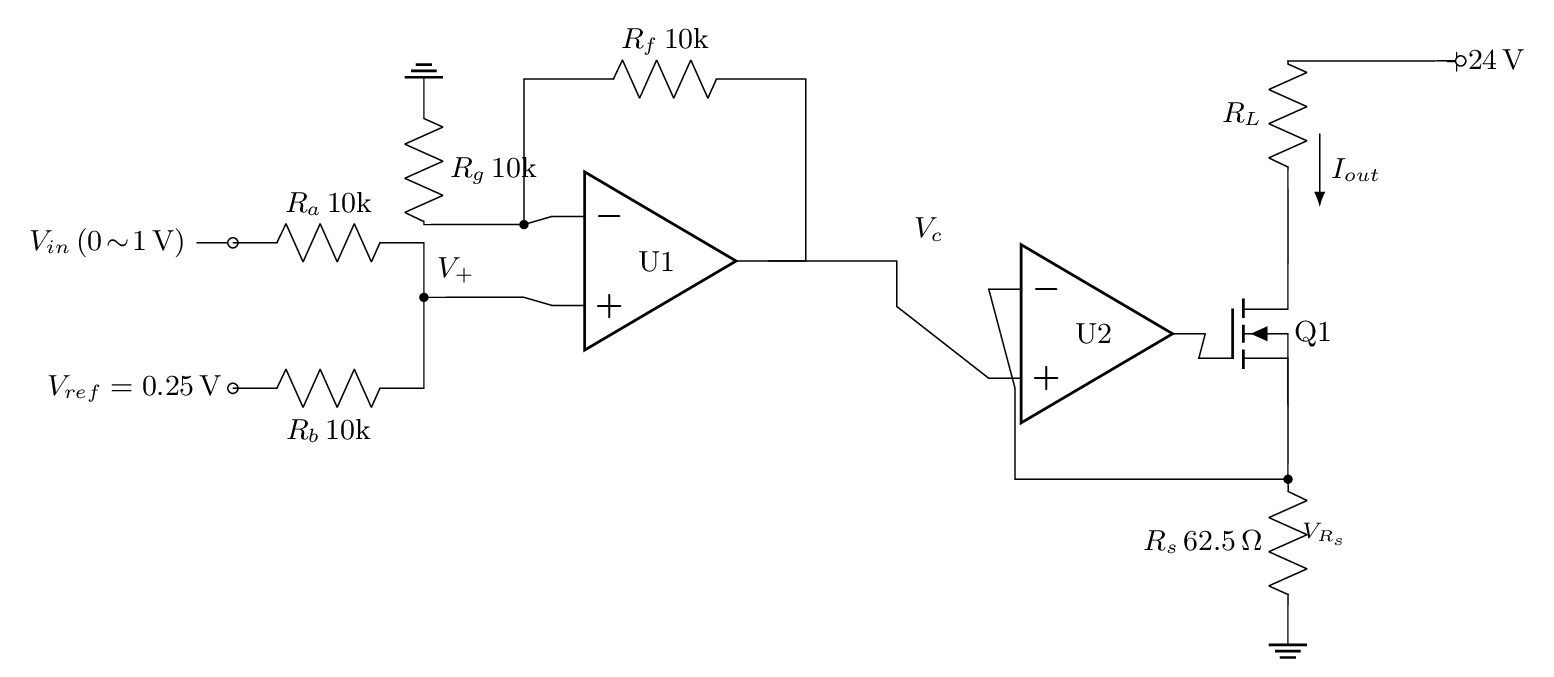
\includegraphics[width=0.95\linewidth]{vi_circuit.png}
  \caption{0\,$\sim$\,1\,VDC 转 4\,$\sim$\,20\,mA 电流输出电路原理图}
  \label{fig:vi}
\end{figure}

\subsection{转换关系验证}
将各输入电压代入，得表~\ref{tab:vi}，输出严格落在 $4\!\sim\!20\,\mathrm{mA}$，且线性。

\begin{table}[htbp]
  \centering
  \caption{输入电压与输出电流对照}
  \label{tab:vi}
  \begin{tabular}{cccccc}
    \toprule
    $V_{in}$ / V & 0 & 0.25 & 0.50 & 0.75 & 1.00 \\
    \midrule
    $V_c=V_{in}+0.25$ / V & 0.25 & 0.50 & 0.75 & 1.00 & 1.25 \\
    $I_{out}=V_c/62.5\,\Omega$ / mA & 4 & 8 & 12 & 16 & 20 \\
    \bottomrule
  \end{tabular}
\end{table}

\subsection{元件选型与注意事项}
\begin{enumerate}
  \item \textbf{运放}：选低失调、低漂移精密运放（如 OP07、OPA2277），减小零点误差；若单 $+24\,\mathrm{V}$
        供电，宜用轨到轨、输入含地的型号。
  \item \textbf{调整管}：优先用 N 沟道 MOSFET（如 2N7000），栅极电流近似为零，
        不引入基极电流误差；若用 NPN 三极管需考虑 $\beta$ 有限带来的误差。
  \item \textbf{取样电阻 $R_s$}：直接决定精度，应选 $0.1\%$、低温漂金属膜电阻，并满足功率
        （$I_{out}^{2}R_s\approx 20\,\mathrm{mA}^2\times 62.5\,\Omega\approx 25\,\mathrm{mW}$）。
  \item \textbf{基准源}：用 TL431/REF3025 等精密基准提供稳定的 $V_{ref}$，保证零点稳定。
  \item \textbf{供电与负载能力（顺从电压）}：$4\!\sim\!20\,\mathrm{mA}$ 环路一般用 $+24\,\mathrm{V}$
        供电。满量程 $20\,\mathrm{mA}$ 时须满足
        $24\,\mathrm{V}\ge I_{out}R_L+V_{R_s}+V_{DS(\min)}$，据此可带最大负载
        $R_{L,\max}\approx\dfrac{24-1.25-V_{DS(\min)}}{20\,\mathrm{mA}}\approx 1\,\mathrm{k}\Omega$。
  \item \textbf{保护}：输出端加反接保护及限压/限流保护，提高现场可靠性。
  \item \textbf{集成方案}：工程上也可直接选用专用电压/电流变送 IC（如 XTR110、AD694、RCV420），
        内部集成基准与零点/量程电阻，只需少量外接元件即可完成 $0\!\sim\!1\,\mathrm{V}\to 4\!\sim\!20\,\mathrm{mA}$
        转换，精度与稳定性更高。
\end{enumerate}

\end{document}
